\documentclass[10pt,twocolumn,letterpaper]{article}
\usepackage[utf8]{inputenc}
\usepackage{hyperref}
\usepackage{amsmath}
\usepackage{subcaption}
\usepackage{graphicx}
\usepackage{booktabs}
\usepackage{lipsum}      
\usepackage{xargs}  
\usepackage[colorinlistoftodos,prependcaption,textsize=medium]{todonotes}

\title{Predicting NCAA Football Game Scores}
\author{Chi Jin \\
Michigan State University \\
{\tt\small jinchi@msu.edu}
\and
Connor Masini\\
Michigan State University\\
{\tt\small masinico@msu.edu}
\date{December 7th, 2018}
}

\begin{document}

\maketitle
\begin{abstract}

College football is one of the most popular sports to watch and bet on in America. Two facets of the game are commonly used for betting: the point differential between the two opposing teams (the point spread) and the total number of points scored collectively by both teams (the over/under). Both these values can be extracted from the final score of the game. We attempted to use a genetic algorithm to train a neural network to predict the final scores of college football games. Through the evolution of neural network hyper-parameters, we were able to create a multilayer perceptron that could predict NCAA football scores at a level comparable to Las Vegas predictions.

\end{abstract}

\section{Introduction}
American football, also known as football or gridiron, is the most popular team sport game in the United States \cite{favsport}, attracting hundreds of millions of people all around the world to an ever-growing fan base.  Between 2010 and 2013, an estimated average of 3.75 million people played football in some form of organized league \cite{ncaa}.
 
Like all popular sports, football has a prosperous betting market.  Both the bookmakers and the bettors wish to make money by betting on the right team.  Before each major football game, a predicted point spread is generated.  Bettors can bet whether the total number of points scored between the two teams is higher or lower than a value determined by the bookmakers (the over/under) or on whether the difference in scores between the two teams (the point spread) will be higher or lower than the bookmakers prediction.  Therefore, the prediction of the game scores is critical for betting in bookmaking business as both major forms of betting rely on the final scores for the games.

From an academic standpoint, this task can test various mathematical methods of prediction and extrapolation as a benchmark \cite{forcast}.  Due to the high turnover rate in college football (players can only play for a maximum of 4 years), the performance of any given team can vary drastically from year to year.  The high turnover rate limiting the usefulness of previous years data in addition to the limited number of games each team plays makes the prediction of college football scores a very interesting and difficult problem.  

\section{Previous Work}
There has been a large amount of work done towards accurately predicting the scores of football games.  This can be attributed to the popularity of the sport in America in addition to the potential monetary gain associated with successfully classifying game scores.  However, one important distinction about this work needs to be stated: most of the research completed has been done on NFL teams instead of NCAA teams.  Predicting NCAA football scores is a much more difficult task than predicting NFL scores, due to the vastly greater number of teams and smaller amount of games in college football \cite{blaikie2011nfl}.  However, the principles used for predicting professional football should also apply to college football.  Many previous studies have utilized artificial neural networks to a great degree of success in predicting the outcome of professional football games \cite{blaikie2011nfl,david2011nfl,purucker1996neural}.  In addition, the usage of genetic algorithms to tune neural network parameters and hyper-parameters is a common practice that can be used to effectively optimize parameters and hyper-parameters \cite{bashiri2011tuning}.  Previous studies have also found that the outcome of any given football game can be predicted with a high probability using 4 statistics: total yards gained, rushing yards gained, turnover margin, and time of possession \cite{purucker1996neural}.  The largest players in predicting game scores are the casino's in Las Vegas. These casino's make money by accurately predicting game results and charging a small fee for individuals to place bets on their preferred teams.  Much of the bench-marking we do to evaluate our performance is in comparison to Vegas Insider (a popular betting website) spreads and over/under point totals \cite{vegas}.

\section{Data}
The data used for this report has already been gathered and is hosted on the Seldom Used Reserve website \cite{SeldomUsedReserve}.  This data set contains detailed game information for every game occurring in the 2011-2018 seasons.  This data set contains box score information about every game.  From the box score data, we are able to generate several advanced statistics about each team's relative strength.
\subsection{Time-Frame}
One problem with datasets drawn from college sports is the unreliability of past seasons data for predicting current performance.  Players can play no more than 4 years for a given NCAA team.  Additionally, many players see limited play-time (in many cases no time) during their first year or two.  This limits the usability of past seasons data towards predicting upcoming games.  However, it is also important to use some of this past data.  Many schools consistently do well year-after-year while other teams consistently place towards the bottom of the NCAA.  In order to effectively predict games occurring towards the beginning of the season, we chose to use data from the previous year while compiling statistics for each team.  This 2-year time-frame was chosen because teams lose an average of 8.16 out of 22 total starters each season, making 1 season the furthest we can go back while the majority of the starters in the league are the same \cite{starters}.

\subsection{Basic Statistics}
We began our feature selection by looking at the basic box-score statistics.  For each team, we compiled a set of offensive statistics present in our database.  These included the number of plays, average yards per play, and total number of yards gained for both pass-plays, run-plays and the combination of the two types of plays.  We also included statistics for penalty yards given up, number of turnovers committed, and time of possession.  For each offensive feature there is a corresponding and opposite defensive feature.  For example, total yards gained is an offensive feature with total yards allowed is the corresponding defensive feature.  All basic statistics were taken as a per-game average to avoid underrating teams that played less games due to weather-based cancellations.  A summary of all basic statistics used can be found in Table \ref{tab:basic_stats}.
\begin{table}
\begin{tabular}{l l}
\hline
Offensive Statistics & Defensive Statistics\\\hline
Passing Yards Gained & Passing Yards Against\\
Pass Plays Attempted & Pass Plays Attempted Against\\
Yards Per Pass & Yards Per Pass Against\\
Run Yards Gained & Run Yards Against\\
Run Plays Attempted & Run Plays Attempted Against\\
Yards Per Run & Yards Per Run Against\\
Total Yards Gained & Total Yards Against\\
Total Plays Attempted & Total Plays Attempted Against\\
Yards Per Play & Yards Per Play Against\\
Penalty Yards & Penalty Yards Against\\
Turnovers Committed & Turnovers Received\\
Time of Possession & Time of Possession Against\\
Points Scored & Points Allowed\\
\hline
\end{tabular}
\caption{\label{tab:basic_stats} List of the basic features derived from the 2-season averages of NCAA football team statistics.}
\end{table}

\subsection{Advanced Statistics}
In order to produce the best possible set of data for our model to work with, we used the set of basic statistics we gathered and combined them to create some advanced metrics that are historically indicative of team success.  These advanced metrics include Glicko scores (A scoring system based on the ELO rating system for chess players), Pythagorean Expectation, Strength of Schedule, win percentage, opponents win percentage, and opponents opponents win percentage.  We also calculated a weighted win percentage (WWP), with away wins weighted more heavily than home wins.
\begin{small}
$$\textrm{WWP} = \frac{\textrm{home wins}*.6 + \textrm{away wins}*1.4 + \textrm{neutral wins}}{\textrm{total games}}$$
\end{small}
This weighted win percentage was then used to calculate Ratings Percentage Index (RPI) using a weighted average of each team's weighted win percentage (WWP), opponent's win percentage (OWP), and opponent's opponent's win percentage (OOWP) as shown below.
\begin{small}
$$\textrm{RPI} = (\textrm{WWP} * 0.25) + (\textrm{OWP} * 0.50) + (\textrm{OOWP} * 0.25)$$
\end{small}
\subsection{Data Collection}
To generate the data matrices that we fed into our neural network, we first ordered all the games in our dataset by date.  Once ordered, we went through each game in the season prior to the one we were trying to predict and compiled averages for each team for each of our basic box score statistics.  Once we processed all games prior to the season we were attempting to predict, we began stepping through the dataset game by game.  For each game, we first compiled a vector representing all of the basic and advanced stat averages per game for each of the two teams in the game.  After this vector was compiled, it was added to our data matrix and the resulting scores for each of the two teams in the game were added to our results matrix.  After adding these rows, we updated the statistics for each team to include their performances in the given game.  Once we processed every game in the given season, we serialized the matrix and appended it to a master data matrix that contained statistics and results for every game between the 2012 and 2018 seasons.

\begin{figure*}[h]
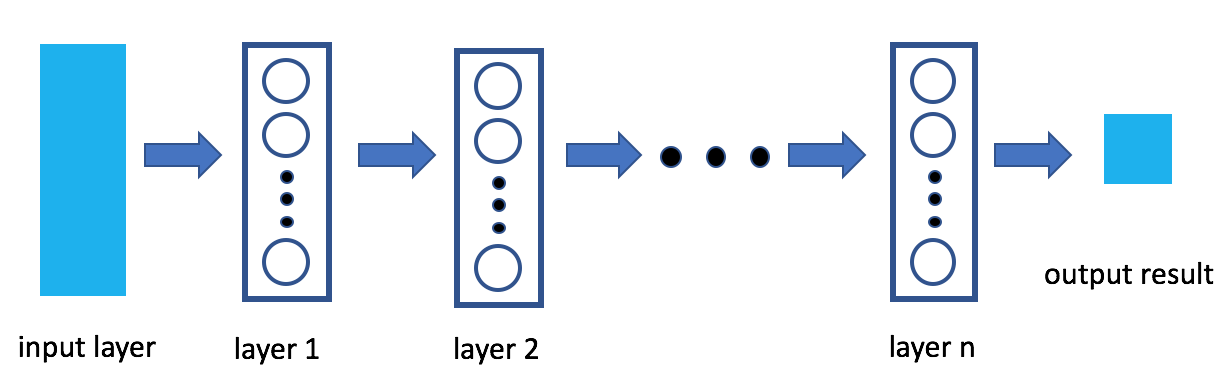
\includegraphics[width=16cm, height=5.4cm]{MLP}
\caption{\label{MLP}Architecture of the MLP model}
\end{figure*}
\section{Methods}

\subsection{Genetic Algorithms}
Genetic algorithms (GAs) have long been developed for prediction tasks like predicting upcoming weather patterns or protein structures \cite{mitchell1995genetic}.  Specifically, GAs are used to evolve machine learning system parameters, like weights and hyper-parameters, like learning rate, number and dimensionality of layers, or number of neurons of a neural network.  In our experiment, we developed a multilayer perceptron model, of which four hyper-parameters are tuned by GAs: number of layers, number of neurons per layer, activation functions and the model optimizer.

\subsection{Representation and Initialization}
Each individual in our population consisted of a set of 4 hyper-parameters.  These parameters include the number of neurons per layer from the set \{16,32,64,128\}, the number of layers out of \{1,2,3,4\}, an activation function from \{ReLU, ELU, TanH, Sigmoid\}, and an optimizer from \{RMSprop, Adagrad, Adadelta, Adam, Adamax, Nadam\}. Initially, we also considered the stochastic gradient descent (SGD) optimizer but found that it occasionally led to NaN values for score predictions and had sub-par performance otherwise. These factors led us to remove the SGD optimizer from our possible genotypes. To initialize the population, we chose a random subset of these values for each our individuals.  We used a population size of 20 for our experiment.
\subsection{Crossover and Mutation}
We designed both crossover and mutation operators for our algorithm.  Mutation consisted of selecting a random hyper-parameter to mutate and setting its value to one of the possible choices for that parameter at random.  Crossover occurs by taking two random individuals in the population that will breed and produce two children.  Each parent has a 50\% chance of passing down any one of their hyper-parameters onto their children and each child consists of a random combination of its two parents hyper-parameters.  For our algorithm, mutation occurs after crossover with a 20\% chance.

\begin{table*}
\begin{tabular}{lcc}
\hline
Statistic&Our predictor & Vegas Predictor\\\hline
Winners picked correctly & 71.8\% & 74.9\%\\
Average point spread difference & 17.2 & 19.2\\
Average over/under difference & 14.0 & 13.4\\
\hline
\end{tabular}
\caption{\label{tab:vegascomp} Long-term average comparison of our predictor with Vegas.}
\end{table*}

\begin{table*}
\begin{tabular}{llccc}
\hline
Team 1 & Team 2 & Score & Our Prediction & Vegas Prediction\\\hline
Ohio State & Northwestern&45-24&34.0-21.6&40.25-23.75\\
Alabama&Georgia&35-28&39.6-20.0&38-26\\
Washington&Utah&10-3&32.1-31.6&24.75-20.25\\
Texas&Oklahoma&27-39&16.4-37.5&35.5-44.5\\
Clemson&Pittsburgh&42-10&37.5-16.4&41-13\\
\hline
\end{tabular}
\caption{\label{tab:casestudyscores} Actual scores, our predicted scores, and the Vegas predictions for all 2018 power 5 conference championship games.}
\end{table*}

\subsection{Fitness}
In order to evaluate the fitness of our individuals we created two fitness functions, one for regular individuals and another for games that result in ties.  Our fitness function was designed so that it encouraged accurate spread and over/under predictions.  The full fitness function can be seen in Figure \ref{eq:fitness}, where $score_p(t)$ represents the predicted score for team $t$ and $score(t)$ represents the actual score of team $t$.
\begin{small}
\begin{align*}
fitness = 
\begin{cases}
\frac{\frac{score_p(t_1) - score_p(t_2)}{score_p(t_1) + score_p(t_2)}}{\frac{score(t_1) - score(t_2)}{score(t_1) + score(t_2)}}\textrm{if } score(t_1) - score(t_2) \neq 0\\
1 - \left|\frac{score_p(t_1) - score_p(t_2)}{score_p(t_1) + score_p(t_2)}\right|
\end{cases}
\end{align*}
\end{small}
\begingroup\vspace*{-\baselineskip}
\captionof{figure}{\label{eq:fitness}Fitness Function}
\subsection{Overview of Genetic Framework}
Our genetic algorithm ran for a total of 20 generations.  To determine which individuals would comprise the next generation, we first discarded the least-fit half of the current population.  Remaining members of the population were then selected with a 50\% chance to survive onto the next generation.  Once the surviving individuals were selected, they were paired together randomly and bred until the population size reached its original size.

\subsection{Neural Network Motivation}
The input data for our neural network is a matrix with a set of statistics for each team playing in each game as the row vectors.  Therefore, the number of rows in the matrix represents the number of games in our training set.  Each feature we extracted from the game statistics is represented by a column in our input matrix. These different features were weighted and combined together using our multilayer perceptron network model.  At our current stage, we didn't explore deep learning models like convolutional neural networks because each sample is only a one-dimensional vector consisting of game statistics that may be not linearly correlated.  Therefore, the local connectivity is not an optimal option directing from adjacent features to the output prediction.

\subsection{Neural Network Structure}
The architecture of our neural network model is shown in Figure \ref{MLP}. The input to the network is the matrix of team statistics for each team prior to each game.  Layers 1 through n are all identical hidden layers with the same input and output dimensionality and activation functions.  The output is a vector of length two representing our predicted final score between the two teams.  

\subsection{Implementation}
We implemented the multilayer perceptron using the Keras library running on top of the Tensorflow framework.  The input layer and all the hidden layers are dense layers.  A singular dropout layer with dropout=0.2 was added between the last hidden layer and the output layer to reduce overfitting.
\section{Results}
Overall, we had a mixed set of results.  Each run of our genetic algorithm took upwards of 5 hours to complete 20 generations, making the testing of different parameters of the genetic algorithm difficult.  We achieved reasonably good accuracies for the point spread, the total number of points scored, and the winner of each game. 
\subsection{Fitness Evolution}
We had difficulties evolving fitness for this problem.  Due to the computational complexity of the problem, we were unable to run more than 40 generations at a time.  This limited the amount of evolution that could be done.  Additionally, due to the dramatic changes in fitness that can occur from a single mutation coupled with our relatively low population size, the average fitness for each generation could change by extreme amounts in each generation.  However, the average fitness did improve over time, even though the improvement was slight and far from linear. A graph of our average fitness per generation can be found in Figure \ref{fitness}.  

\begin{figure*}[h]
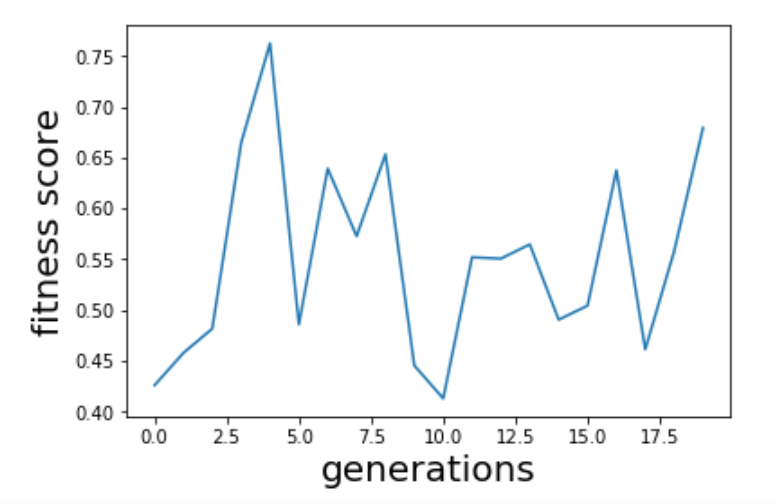
\includegraphics{old_fitness_function.png}
\caption{\label{fitness}Fitness over time}
\end{figure*}

\begin{table*}
\begin{tabular}{llccc}
\hline
Team 1 & Team 2 & Actual Spread & Our Spread & Vegas Spread\\\hline
Ohio State & Northwestern&21&12.4&16.5\\
Alabama&Georgia&7&19.6&12\\
Washington&Utah&7&.5&4.5\\
Texas&Oklahoma&22&21.1&9\\
Clemson&Pittsburgh&32&21.1&28\\
\hline
\end{tabular}
\caption{\label{tab:casestudyspread} Actual point spread, our predicted point spread, and the Vegas point spread for all 2018 power 5 conference championship games.}
\end{table*}

\begin{table*}
\begin{tabular}{llccc}
\hline
Team 1 & Team 2 & Score & Our Prediction & Vegas Prediction\\\hline
Ohio State & Northwestern&69&64&55.6\\
Alabama&Georgia&63&59.6&64\\
Washington&Utah&13&63.7&45\\
Texas&Oklahoma&66&53.9&80\\
Clemson&Pittsburgh&52&53.9&54\\
\hline
\end{tabular}
\caption{\label{tab:casestudyou} Actual total points scored, our predicted over/under, and the Vegas over/under for all 2018 power 5 conference championship games.}
\end{table*}
\subsection{Prediction Statistics and Comparison with Vegas}
For every NCAA football game that occurs, Vegas sets both an over/under and a point spread.  People can then bet whether they think the total scores of the two teams combined will exceed or fall short of the Vegas over/under or whether they think the point differential between the teams will be greater than or less than the Vegas point spread.  Vegas is generally considered one of the most accurate predictors of game outcomes.  If they did not accurately predict games, they would quickly be run out of business as they charge only a slight processing fee for placing bets.  Across our entire dataset, our point spreads were off by an average of 17.2 points, our over/under totals were off by an average of 14.0 points, and we correctly identified the winning team 71.8\% of the time.  These predictions are comparable to the Vegas predictions, which are off by an average of 19.2 points for the point spread, 13.4 points for the over/under total, and predicts the correct winner 74.9\% of the time.  Our spread predictions were slightly better than Vegas's, while our over/under point total predictions and winner predictions were slightly worse.  A summary of this information can be found in Table \ref{tab:vegascomp}.  If we were to have used our model's score predictions to bet on the Vegas over/under, we would have won in 49.98\% of scenarios.  Because there are only two possible choices to bet on (over and under the Vegas point total), each of which is equally likely, our result shows  no significant prediction ability over Vegas's Over/Under.  This makes sense as our predicted Over/Under was less accurate than the Vegas Over/Under throughout our entire dataset.  However, our predictor correctly bet on the Vegas point spread in 51.2\% of games.  Using a 90\% confidence interval, we can conclude that our predictor can predict which side of the point spread to bet on more than half the time.  This is an encouraging result and indicates that our predictor is effective at estimating the point spread between teams.

\subsection{Conference Game Case Study}
As an interesting case-study, we decided to use our predictor to estimate the scores of all the power 5 conference championship games. These match-ups included Ohio State vs. Northwestern, Alabama vs. Georgia, Washington vs. Utah, Texas vs. Oklahoma, and Clemson vs. Pittsburgh. A summary of the actual scores, our predicted scores, and the Vegas predictions for these 5 games can be found in Table \ref{tab:casestudyscores}. Additionally, summaries of the 3 spreads and over/under point totals can be found in Tables \ref{tab:casestudyspread} and \ref{tab:casestudyou}. Overall, our algorithm did a good job predicting scores for these games. It correctly picked every winner and guessed the scores of all but 3 teams within 25\% of the actual score. In particular, the algorithm did an excellent job estimating the point totals of each game, missing by less than 19\% for all but one of the games. The only game that our algorithm failed to reasonably predict was the Washington vs. Utah game. This game was unusually low scoring given both teams history and Vegas also failed to effectively predict the outcome, albeit by a lessor amount than our algorithm.


\section{Future Work}
\subsection{Differentiate hidden layers}
Currently the genetic algorithm was applied to the whole model for selecting the number of layers hyper-parameter. This means that all the hidden layers in any given model have the same hyper-parameters. However, this limits the evolution space.  Intuitively, the hidden layers at different levels sharing the same dimensionality and activation function can hardly work as well as those with more flexibility of selecting number of neurons and the activation function. For example, the deeper layers that are closer to the output layer usually have less neurons than the shallow layers to avoid overfitting and to reduce the computational cost. In the future, we would like to evolve all the hidden layers independently so they can have different dimensionalities and activation functions.

\subsection{Vary the dropout values}
Dropout is a way to reduce overfitting by randomly setting the weights of certain number of neurons in a layer to 0. Currently, we only applied a dropout value of 0.2 to the last hidden layer connected to the output layer. The optimal dropout values for different hidden layers can also be evolved through GA to save computation time and prevent overfitting while maintaining both training and testing accuracies.

\subsection{Test different crossover and mutation rates}
In the experiment, we used a mutation rate of 0.2, a retention rate of 50\%, and a random selection rate of 0.9 for the top 50\% of models based on our fitness function.  These evolution rates could also be optimized by the genetic algorithm to maximize our models performance.

\subsection{Reconsider the fitness function}
Our current fitness function that measured the relative prediction errors may not be optimal. Other prediction statistics measured during the training process can also be used to evaluate the fitness of the models. For example, the accuracy rate of predicting the winning team or the mean difference between actual and predicted scores could be incorporated into a different fitness function.

\bibliographystyle{unsrt}

\bibliography{bibliography.bib}
\end{document}